% appendix.tex
% ============================================================
% Appendix: Additional Regression Results & Supplementary Figures
% ============================================================
\clearpage
\appendix

% ---- 本文上に「Appendix」と表示し、目次にも出す（これが最も確実） ----
\section*{Appendix}
\phantomsection
\addcontentsline{toc}{section}{Appendix}



% ------------------------------------------------------------
% A1, A2... / B1, B2... の番号付け（chngcntr が必要）
% ------------------------------------------------------------
\counterwithin{table}{section}
\counterwithin{figure}{section}
\renewcommand{\thetable}{\Alph{section}\arabic{table}}
\renewcommand{\thefigure}{\Alph{section}\arabic{figure}}


\section{Additional Regression Results}
% ============================================================

\subsection{IV Specifications}

\captionof{table}{2SLS (No Lag)}
\label{tab:A2_iv_nolag}
\input{tables/table_iv_nolag.tex}


\newpage
\captionof{table}{2SLS (Lag 1)}
\label{tab:A3_iv_lag1}
\input{tables/table_iv_lag1.tex}


\newpage
\captionof{table}{Dynamic 2SLS}
\label{tab:A4_dyn_2sls}
\input{tables/table_dyn_2sls.tex}


\subsection{Robustness and Subsamples}
\captionof{table}{2SLS (Lag 1) --- Frontier (Strict)}
\label{tab:A7_iv_lag1_frontier_strict}
\input{tables/54_table_iv_lag1_frontier_strict.tex}


\newpage
\captionof{table}{Dynamic 2SLS --- Frontier (Strict)}
\label{tab:A8_dyn_2sls_frontier_strict}
\input{tables/55_dyn_2sls_frontier_strict.tex}



% ------------------------------------------------------------
% Descriptive table（注意）
% table1_descriptive.tex は現在エラーでコンパイル停止しているため、
% いったんコメントアウト推奨。
% （後でR側で再生成するか、PDF化して \includepdf で貼る）
% ------------------------------------------------------------
% \begin{sidewaystable}[p]\centering
%   \caption{Descriptive Statistics}
%   \label{tab:A10_desc}
%   \InputTable{table1_descriptive.tex}
% \end{sidewaystable}

\clearpage
% ============================================================
\section{Supplementary Figures}
% ============================================================

% ここは「実際に存在するファイル名」に合わせて差し替えてください。
% 例：choropleth / hist / scatter の出力名は 60_figures 系スクリプトに依存。

\subsection{choropleth}

\begin{figure}[!htbp]\centering
  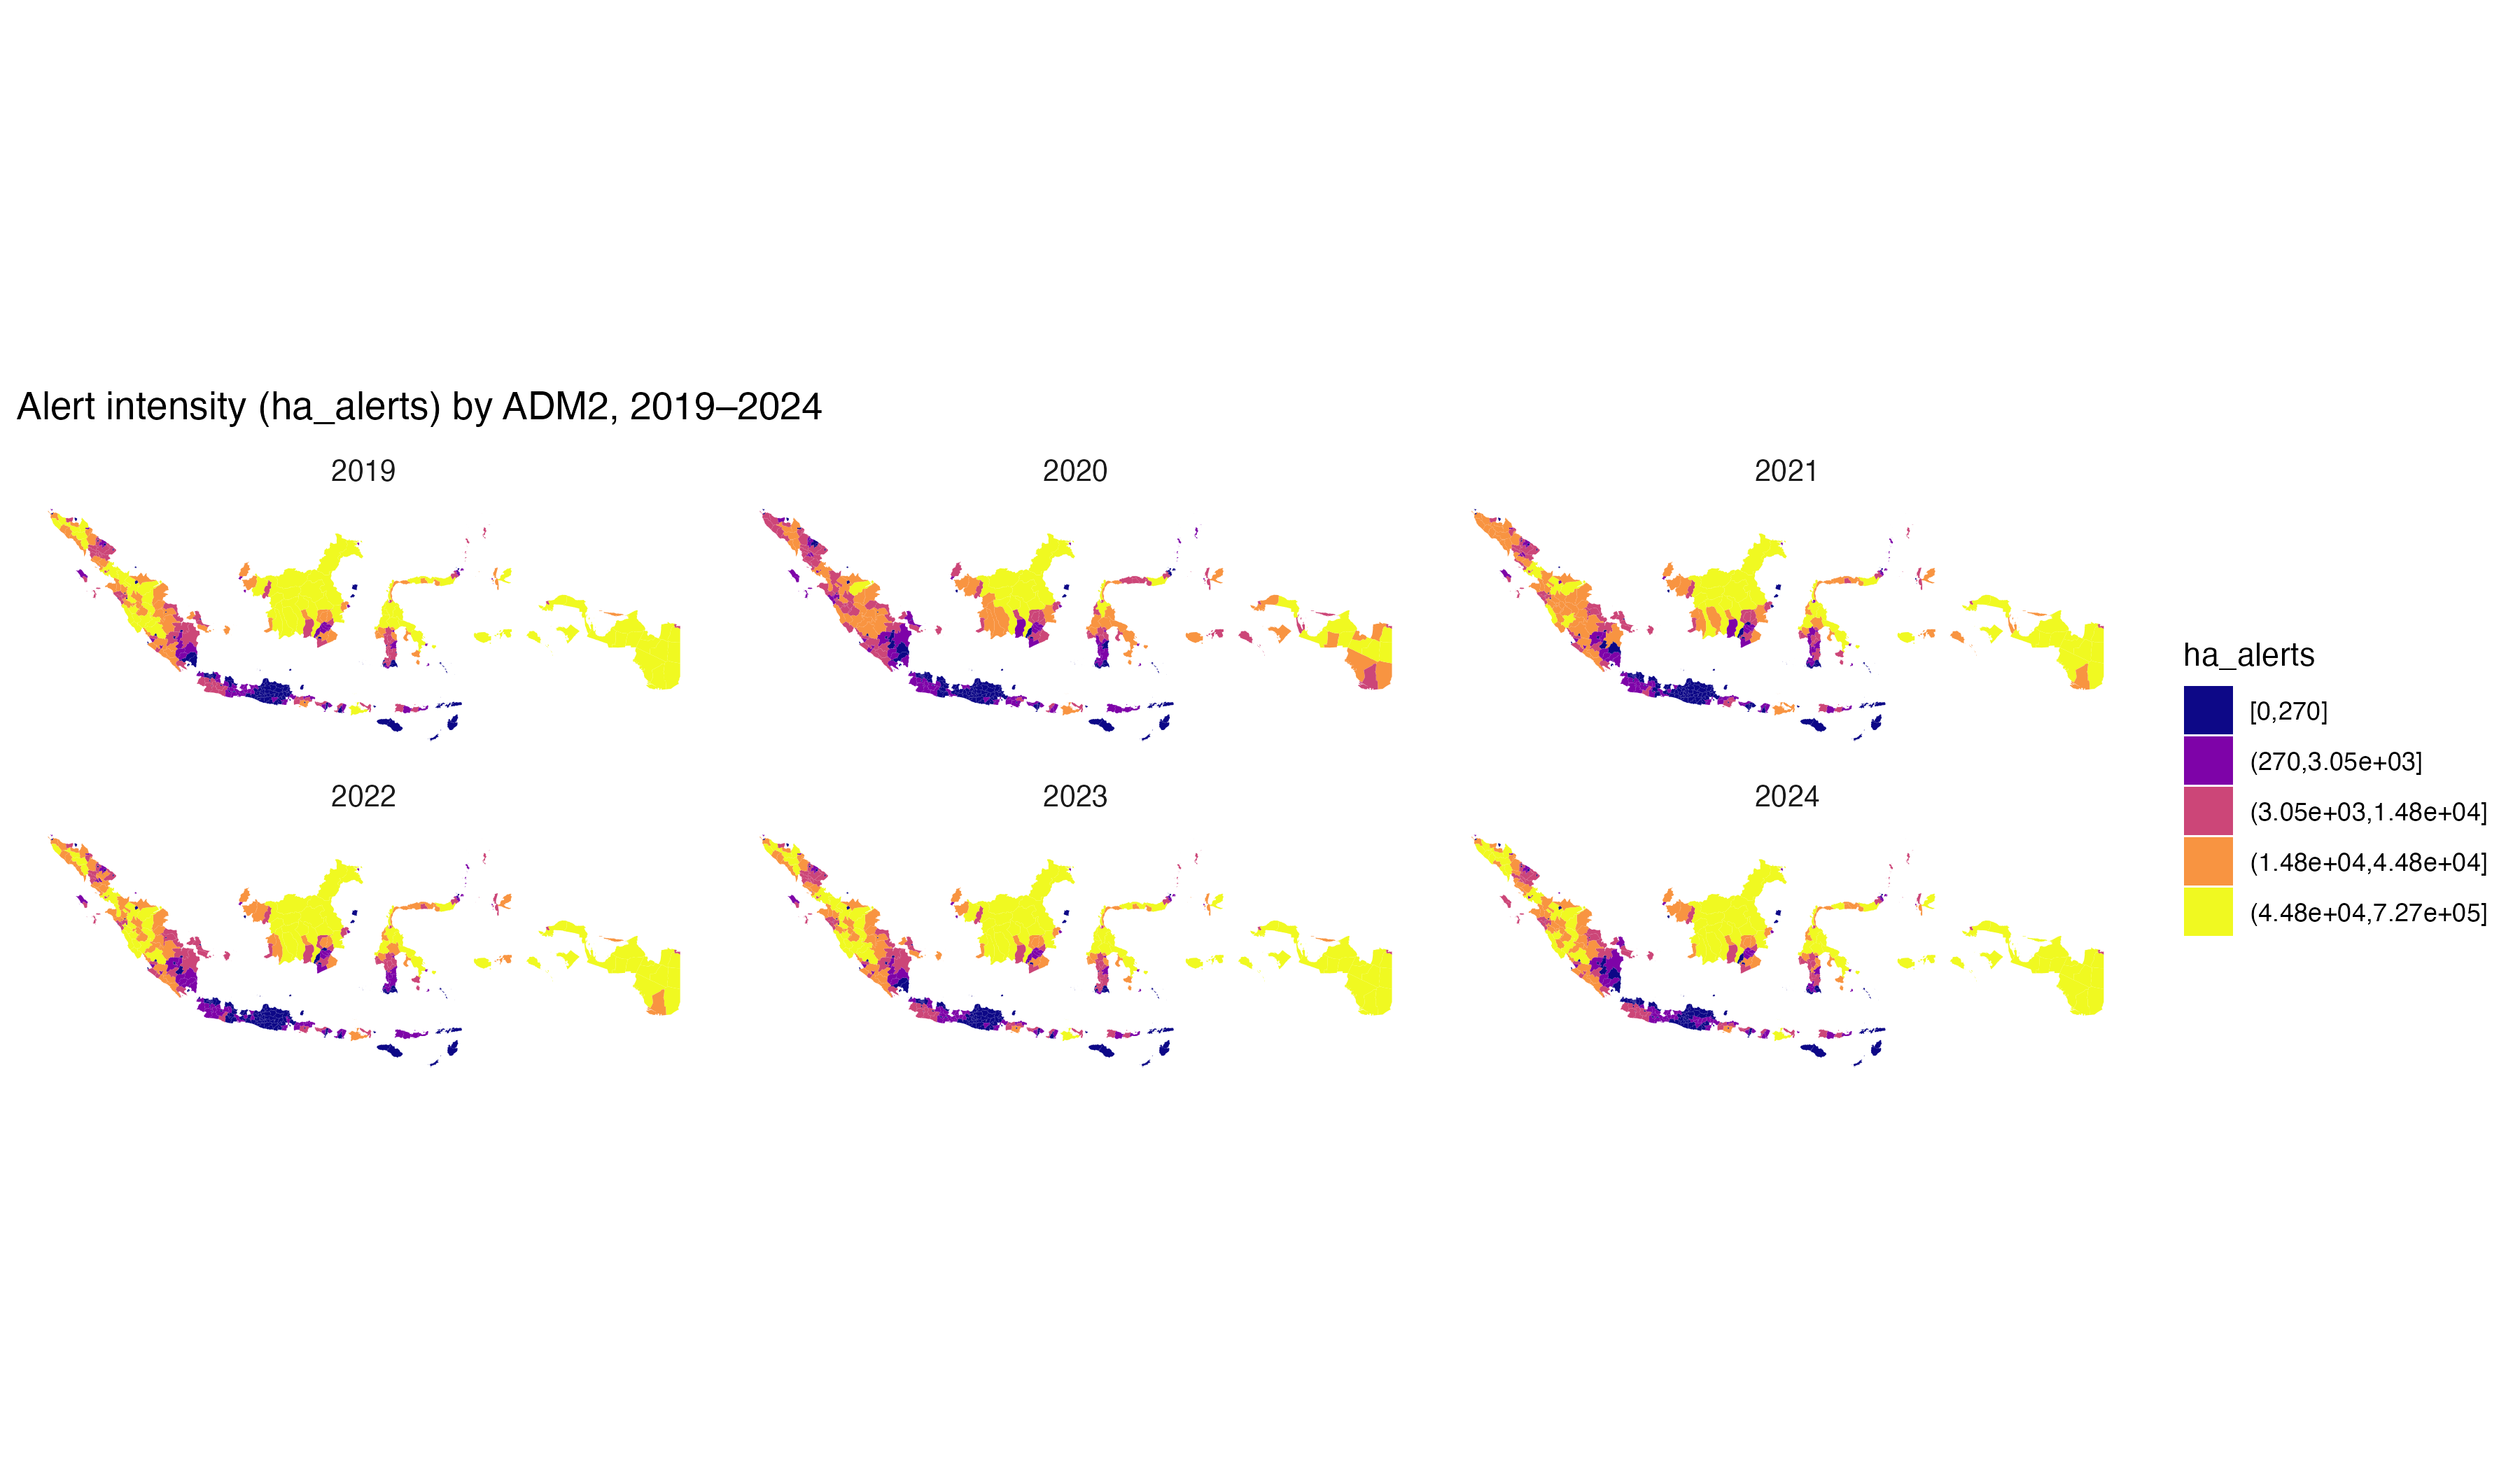
\includegraphics[width=400pt]{figures/choropleth/alerts_intensity_adm2_2019_2024.png}
  \caption{Integrated Alerts Intensity (ADM2, 2019--2024)}
  \label{fig:alerts_map}
\end{figure}

\begin{figure}[!htbp]\centering
  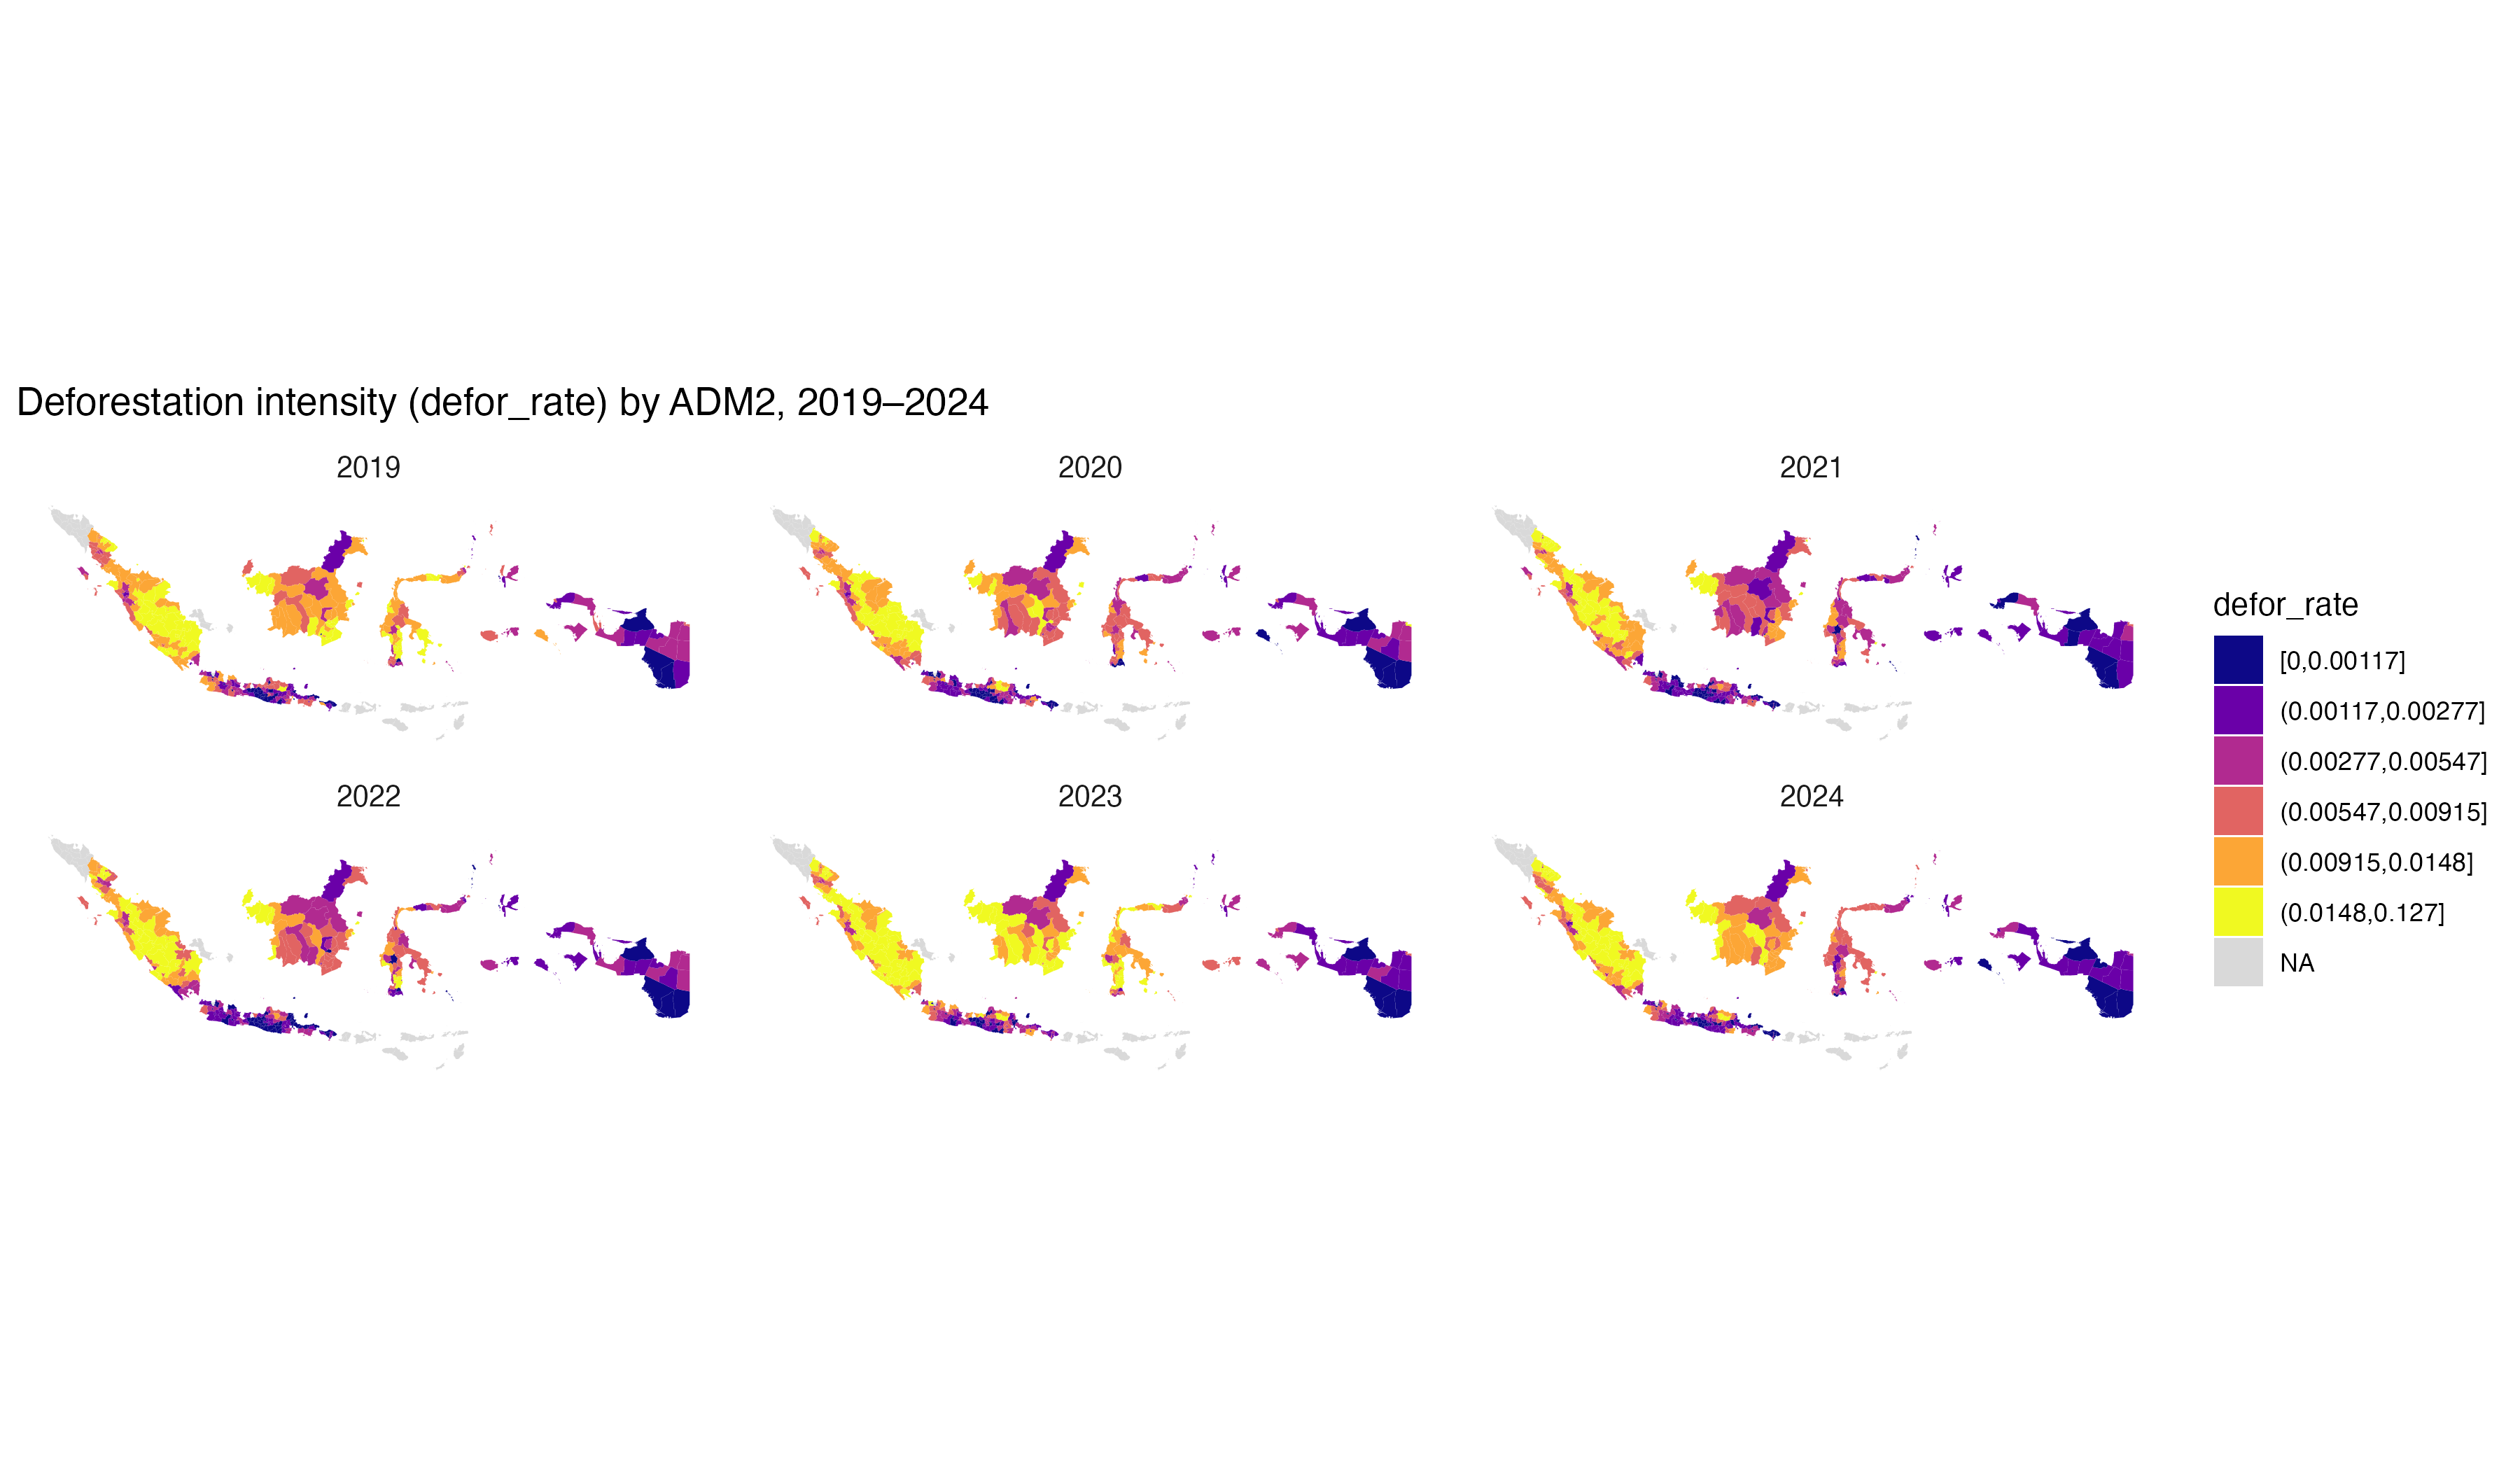
\includegraphics[width=400pt]{figures/choropleth/defor_intensity_adm2_2019_2024.png}
  \caption{Deforestation Intensity (ADM2, 2019--2024)}
  \label{fig:defor_map}
\end{figure}


%%%%%%%%%%%%%%%%%%%%%%%%%%%%%%%%%%%%%%%%
\FloatBarrier
\subsection{Histograms}

\begin{figure}[!htbp]\centering

  % 1行目
  \begin{minipage}{0.49\textwidth}\centering
    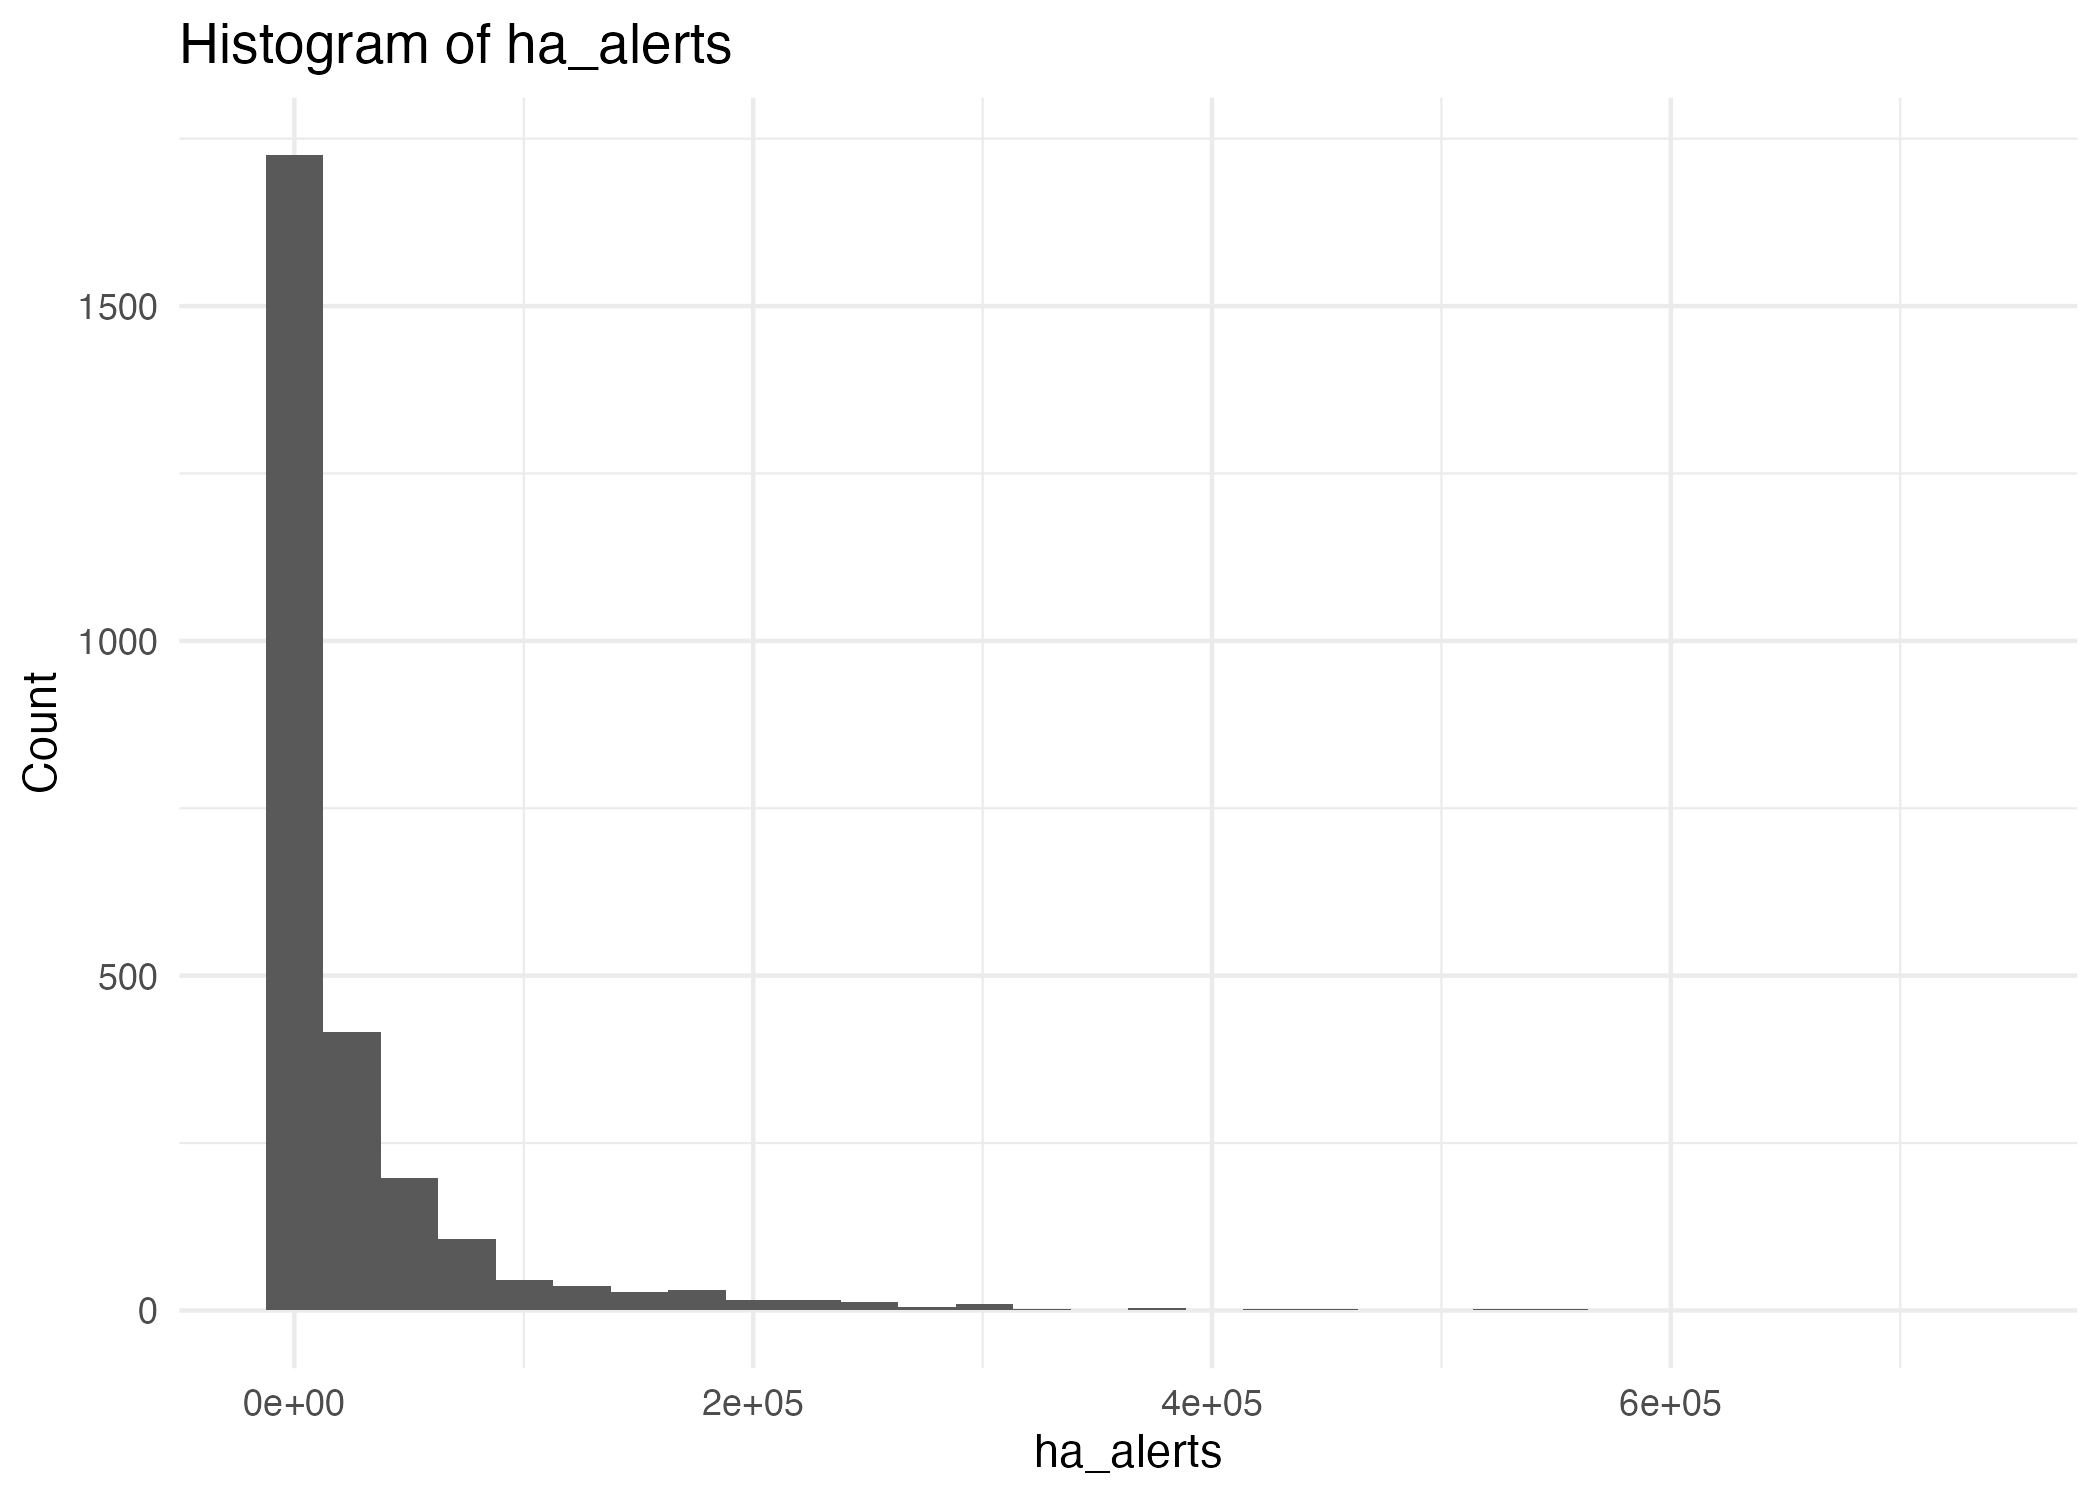
\includegraphics[width=\textwidth]{figures/hist/ha_alerts_hist.png}
    \caption*{(a) Alerts (ha)}
  \end{minipage}\hfill
  \begin{minipage}{0.49\textwidth}\centering
    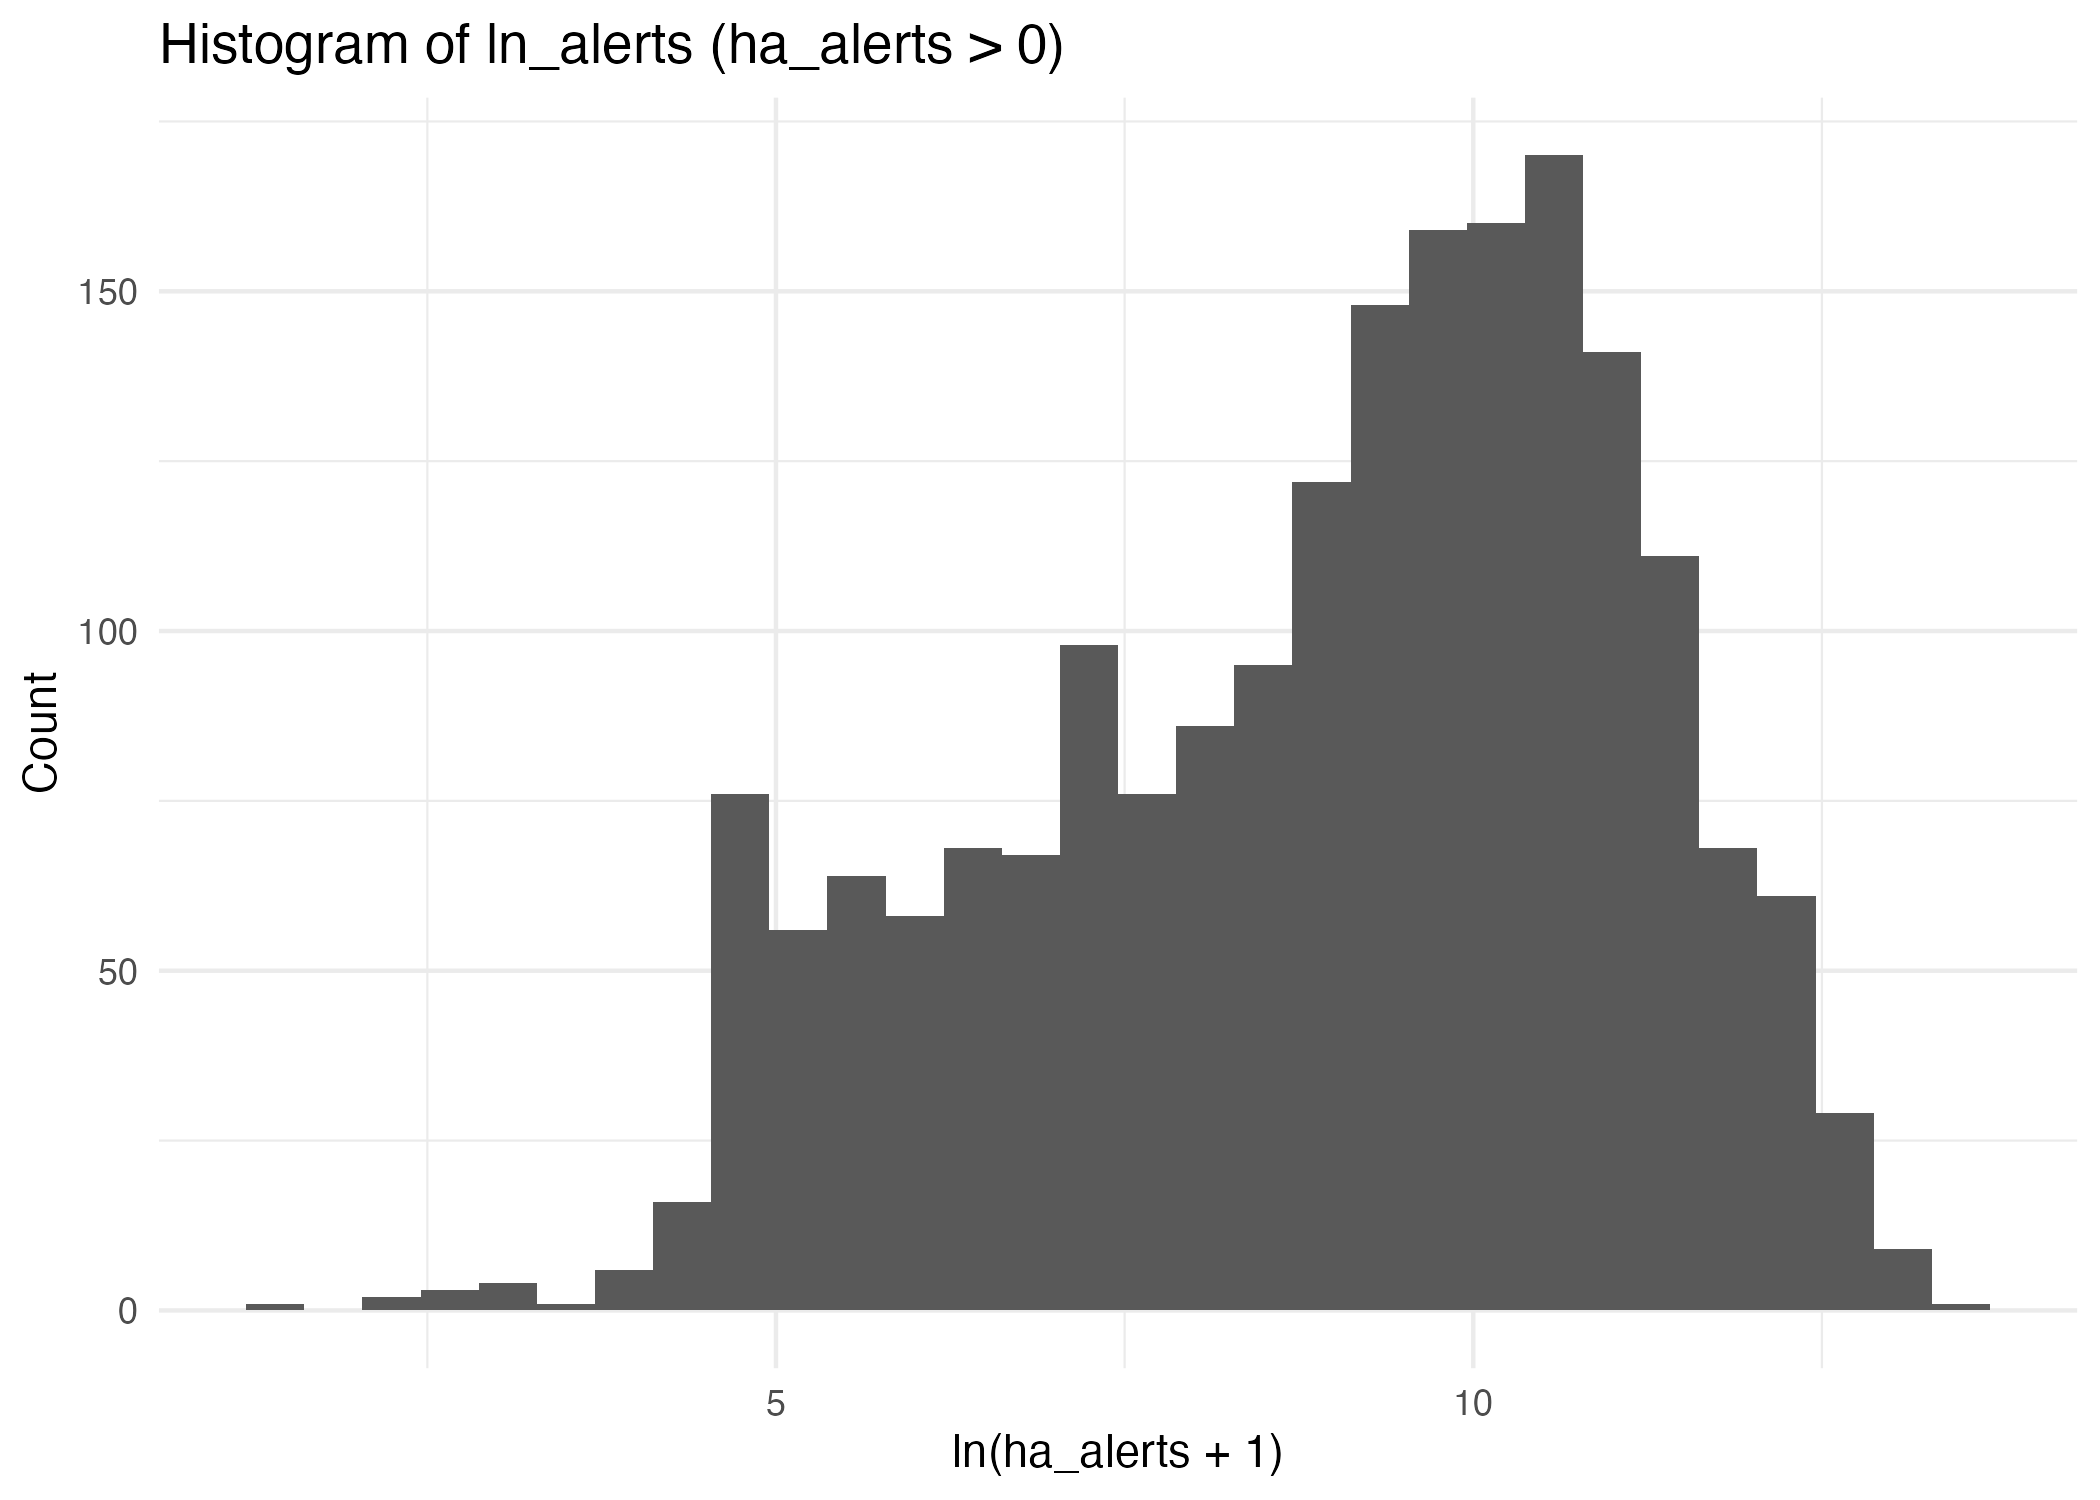
\includegraphics[width=\textwidth]{figures/hist/ln_alerts_hist.png}
    \caption*{(b) $\ln(\text{ha\_alerts}+1)$}
  \end{minipage}

  \vspace{0.6em}

  % 2行目
  \begin{minipage}{0.49\textwidth}\centering
    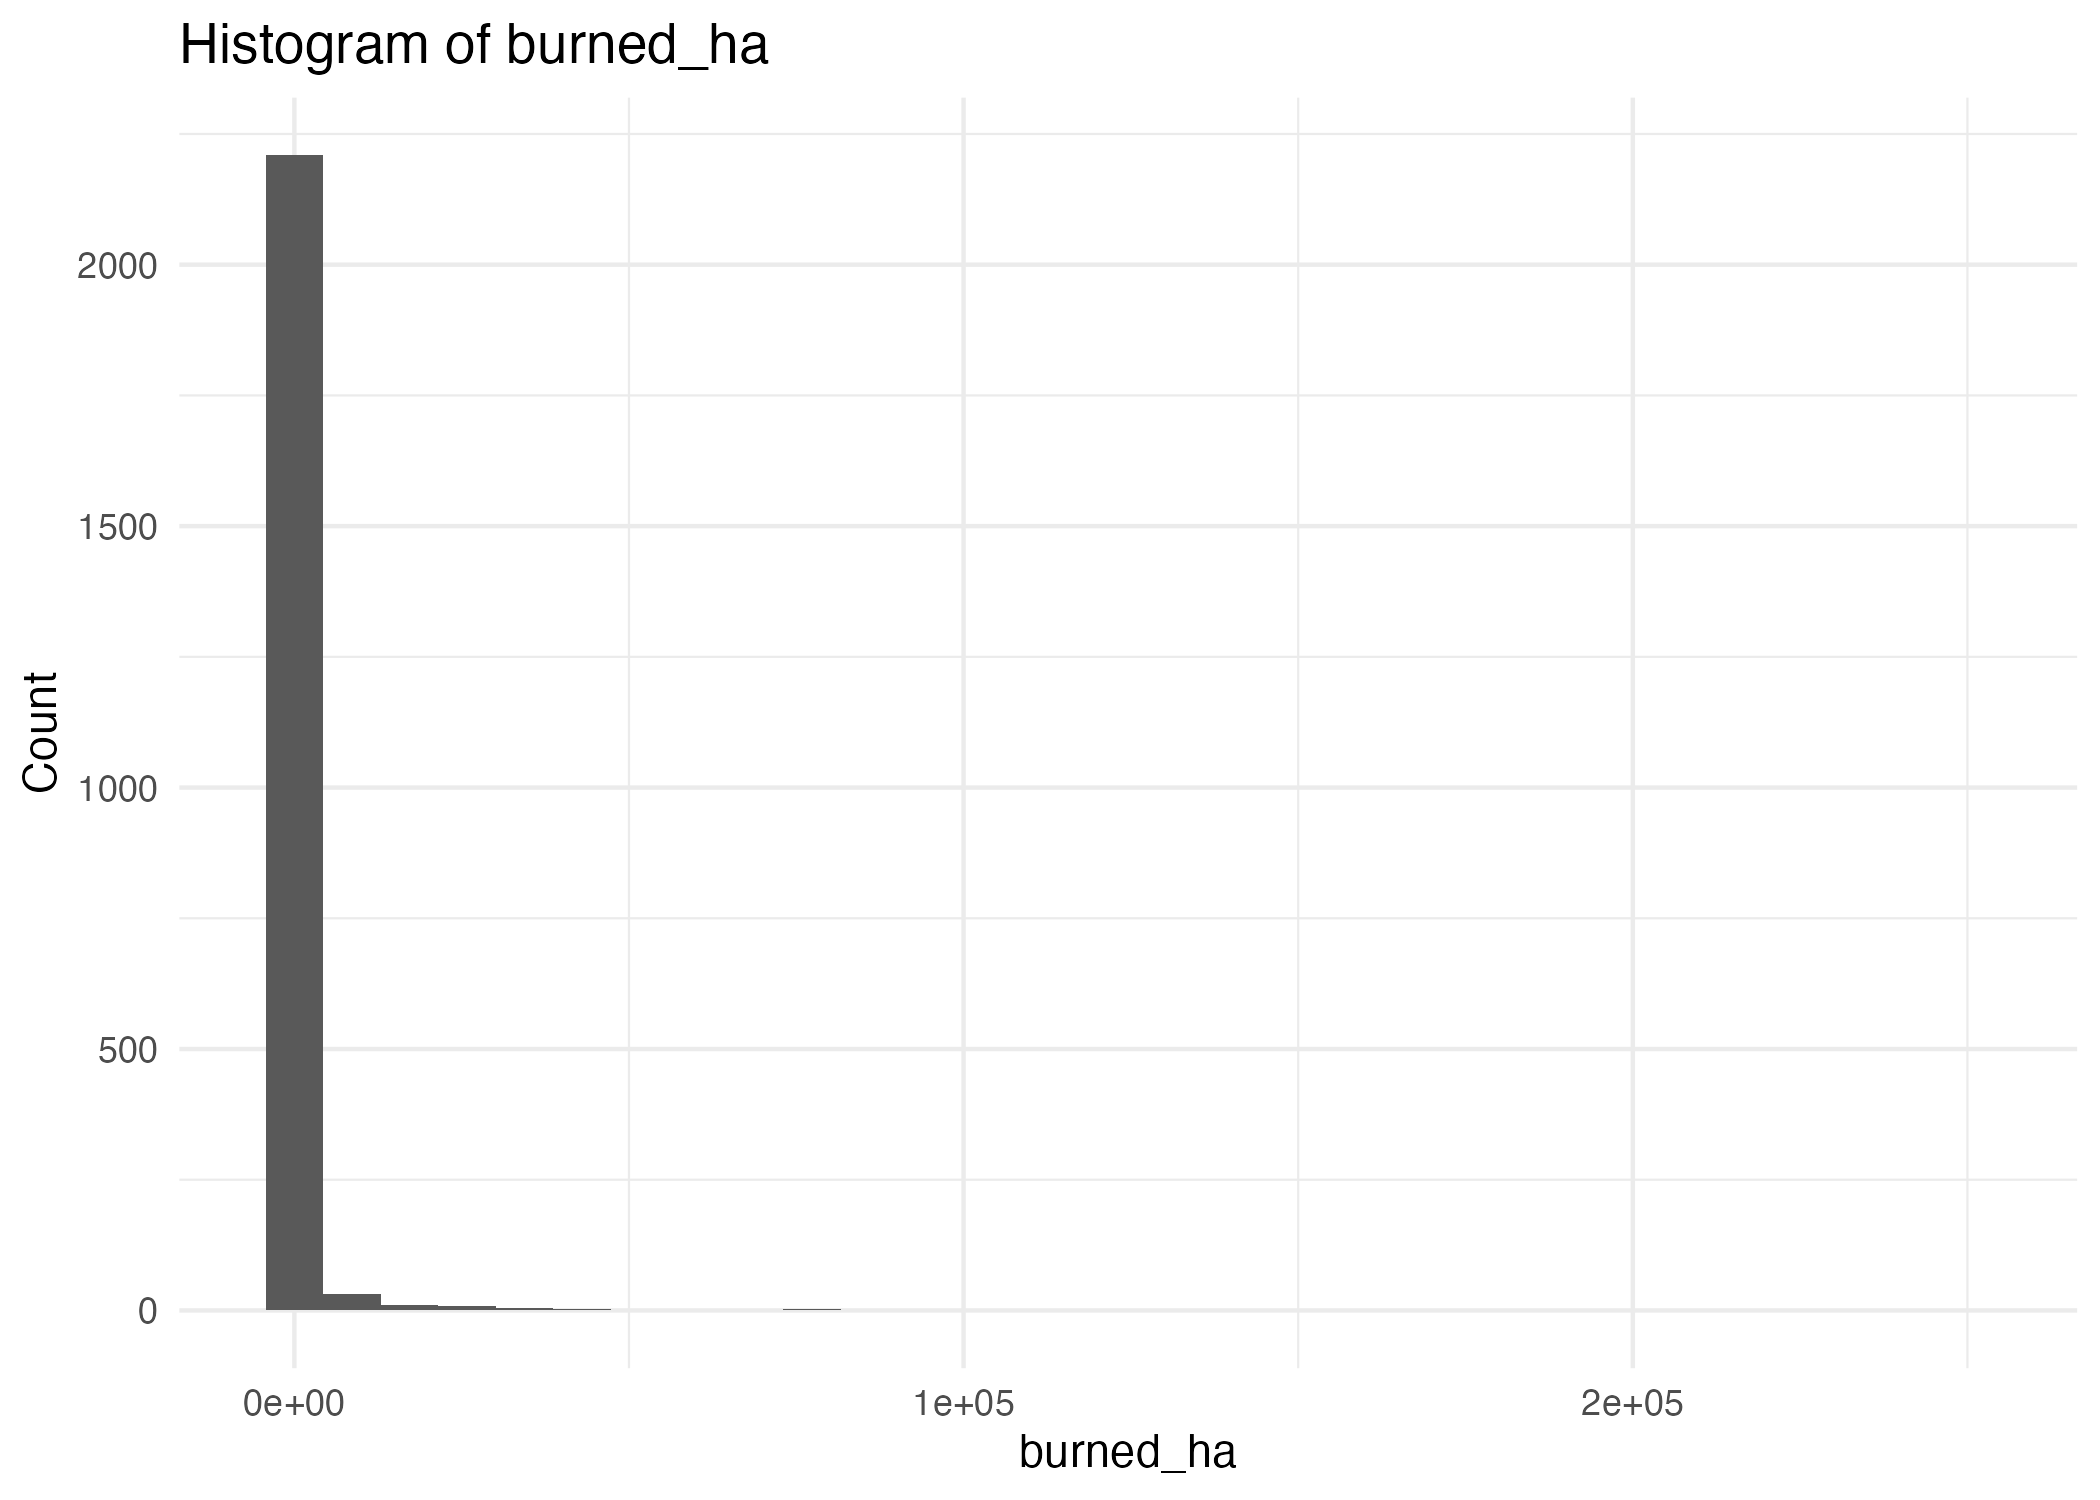
\includegraphics[width=\textwidth]{figures/hist/burned_ha_hist.png}
    \caption*{(c) Burned area (ha)}
  \end{minipage}\hfill
  \begin{minipage}{0.49\textwidth}\centering
    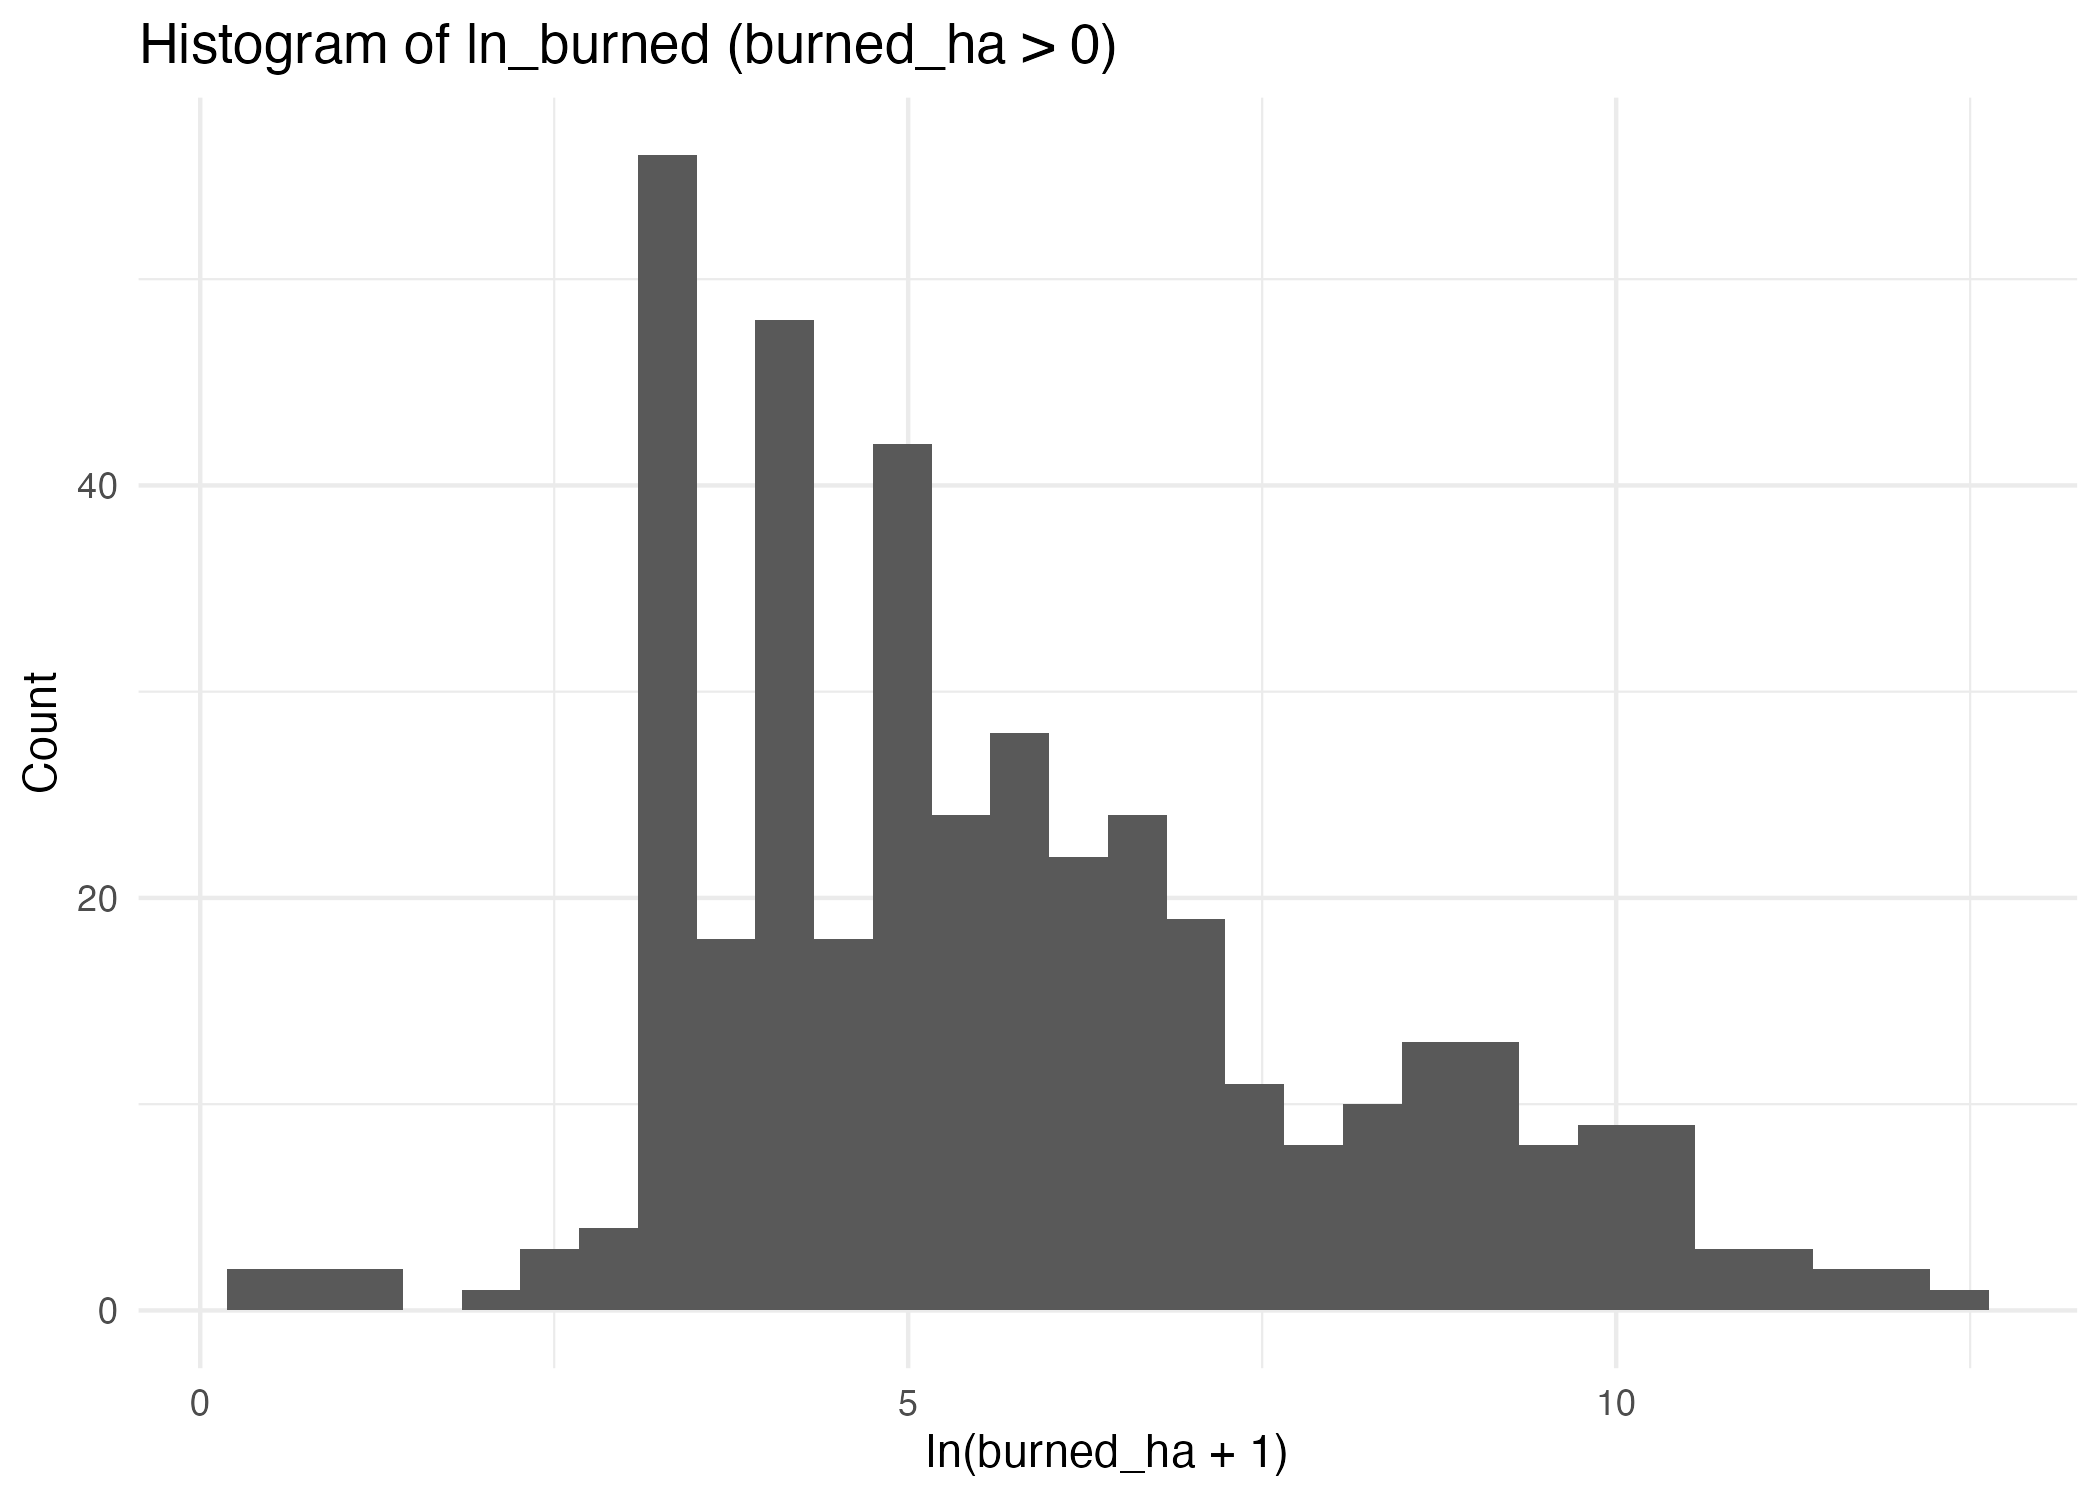
\includegraphics[width=\textwidth]{figures/hist/ln_burned_hist.png}
    \caption*{(d) $\ln(\text{burned}+1)$}
  \end{minipage}

  \caption{Histograms of key variables.}
  \label{fig:appendix_hists}

\end{figure}

%%%%%%%%%%%%%%%%%%%%%%%%%%%%%%%%%%%%%%%%
\newpage
\subsection{Scatterplots}
\begin{figure}[!htbp]\centering
  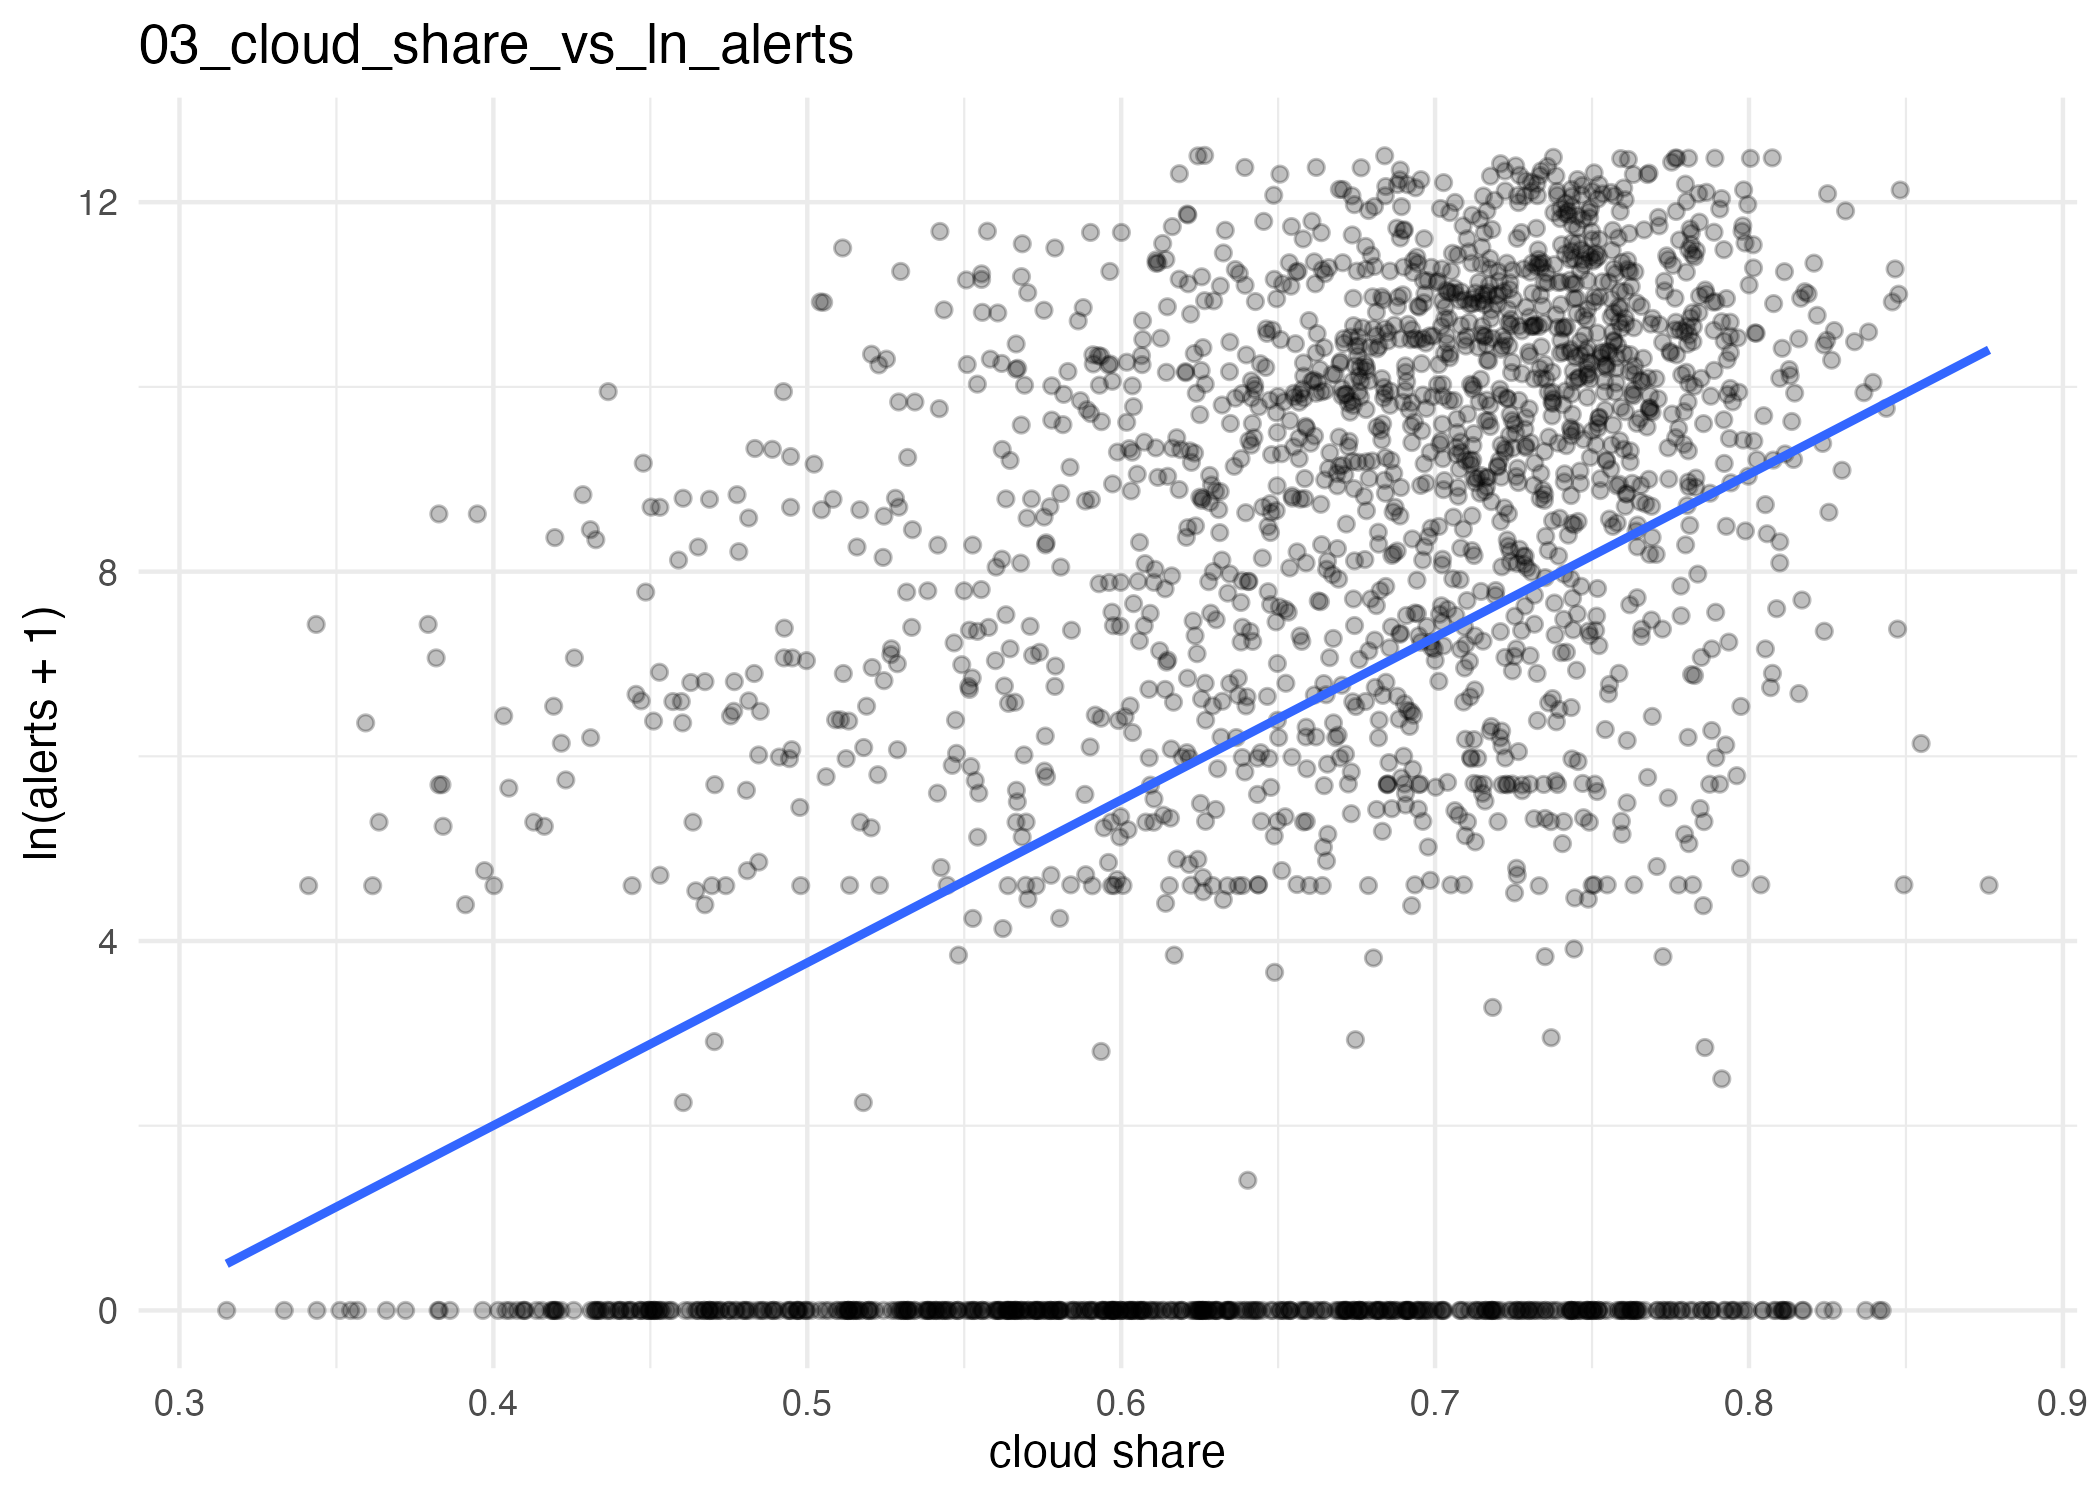
\includegraphics[width=\textwidth]{figures/scatter/03_cloud_share_vs_ln_alerts.png}
  \caption{Cloud Share vs ln Alerts}
  \label{fig:cloud_share_alerts}
\end{figure}

